\section{Multicore}
\subsection{Steigern der Geschwindigkeit eines Prozessors}
Die Geschwindigkeit eines Prozessors kann mit den folgenden Methoden gesteigert werden.

\subsubsection{Clockfrequenz erhöhen}
\begin{itemize}
	\item PCB-Design wird sehr anspruchsvoll  (Leitungslängen, Reflexionen, etc.)
	\item Elektrische Verlustleistung steigt linear mit der Clockfrequenz (Hitzeproblematik)
	\begin{equation}
		P = f_{cl} \cdot C_L \cdot V_{dd}^2
	\end{equation}
	\item Lichtgeschwindigkeit ist die Grenze.
\end{itemize}

\subsubsection{Instruction-level parallelism (ILP)}
\begin{itemize}
	\item Parallelismus wird auf Instruktionslevel angestrebt 
	\begin{itemize}
		\item Pipelines
		\item Verschachteln der Instruktionen, um Pipeline möglichst optimal auszulasten 
		\item Vermeiden von Pipeline flush durch Vorhersage der Verzweigung (branch prediction) 
	\end{itemize}
	\item Branch prediction kann sehr aufwendig werden 
	\item Compiler werden komplex
\end{itemize}

\begin{multicols}{2}
\subsubsection{Thread-level parallelism (TLP)}
\begin{itemize}
	\item Parallelisiert wird auf einer umfangreicheren Stufe als nur auf der Instruktion 
	\item Die parallelisierte Einheit ist in der Grössenordnung einer Funktion 
	\item Zugriffe auf gemeinsame Ressourcen, z.B. sharedmemory, müssen geregelt werden 
	\item Design Issues 
	\begin{itemize}
		\item Nicht einfach beliebig viele Threads spendieren 
		\item Jeder Thread erzeugt Overhead 
		\item Die Threads sollten möglichst unabhängig voneinander sein
		\item Wenn zu viele Threads definiert werden (wenn Zusammengehörendes auseinandergenommen wird), dann werden Daten unnötigerweise shared
	\end{itemize}		
\end{itemize}
\columnbreak
\paragraph{Umsetzung}
\begin{itemize}
	\item Uniprocessor(single-core) 
	\begin{itemize}
		\item Die Threads werden time-sliced 
		\item Pseudo-TLP
		\item Context switch notwendig
	\end{itemize}
	\item  Multiprocessor(Computer mit mehreren Prozessoren) 
	\begin{itemize}
		\item Mehrere parallele Prozessoren können je einen Thread bearbeiten 
		\item Echter TLP 
		\item Clockfrequenzkann tiefer gehalten werden 
		\item Einfachere Hardware wird multipliziert 
		\item Datenaustausch zwischen Prozessoren muss irgendwie geregelt werden, z.B. mit Message Passing oder SharedMemory
	\end{itemize}
\end{itemize}
\end{multicols}
\newpage

\subsection{Multicore Prozessor}
\begin{multicols}{2}
	\begin{itemize}
		\item Ein Multicore Prozessor ist ein spezieller Multiprocessor. Alle Prozessoren (Cores) befinden sich auf demselben Chip
		\item  Multicore Prozessoren sind MIMD (Multiple Instructions Multiple Data). Jeder Core führt einen eigenen Code aus und arbeitet auf unterschiedlichen Daten 
		\item Die Speicherorganisation ist oft komplex
		\item Zwei Typen
		\begin{itemize}
			\item Homogener Multicore Prozessor (mehrere gleiche Cores)
			\item Heterogener Multicore Prozessor (mehrere gleiche/unterschiedliche Cores). Häufig bei Embedded Multicore Prozessoren		
		\end{itemize}
	\end{itemize}
\columnbreak
	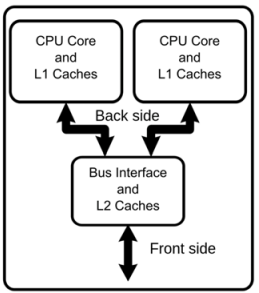
\includegraphics[width=0.4\textwidth]{images/Multicore/Multicore}
\end{multicols}

\subsubsection{Amdahl's Law}
Gesamtaufgabe soll auf möglichst viele Cores aufgeteilt werden, um eine optimale Ausführungszeit zu erzielen. \\
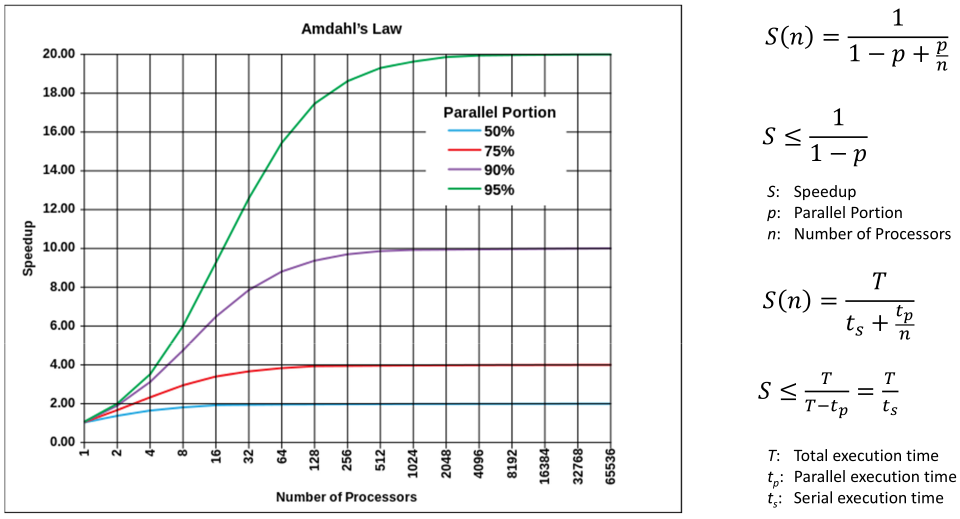
\includegraphics[width=1\textwidth]{images/Multicore/amdahl}

\subsubsection{Speicherorganisation}
\begin{multicols}{2}
	\begin{itemize}
		\item Shared Memory
		\begin{itemize}
			\item Alle Prozessoren nutzen einen gemeinsamen Speicherbereich 
			\item Einfache Implementation 
			\item Shared Memory kann zum Flaschenhals werden 
		\end{itemize}
	\end{itemize}
\columnbreak
	\begin{itemize}
		\item Distributed Memory
		\begin{itemize}
			\item Jeder Prozessor hat seinen eigenen lokalen Speicher 
			\item Für den Datenaustausch unter den Prozessoren muss wiederum ein Mechanismus zur Verfügung gestellt werden, z.B. Message Passing
		\end{itemize}
	\end{itemize}
\end{multicols}

\paragraph{Programmierung von Shared Memory}
\begin{minipage}[c]{14cm}
	\begin{itemize}
		\item Die beiden Cores haben eigene Adressbereiche 
		\item Die Variable \lstinline{sharedVariable} liegt auf einer festen Adresse im Shared Memory 
		\item \lstinline{sharedVariable} wird von beiden Cores genutzt
		\item  Der Zugriff auf \lstinline{sharedVariable} muss synchronisiert werden
		\item Zwischen den CPU Cores und \lstinline{sharedVariable} können mehrere Caches liegen 
		\item Jeder Core muss für sich diese Variable definieren 
		\item Bei \lstinline{int sharedVariable;} darf der Compiler eine Kopie in einem Arbeitsregister anlegen. Unbedingt verhindern!
		\item Die Definition muss zwingend mit \lstinline{volatile} versehen werden: \lstinline{volatile int sharedVariable;}	
	\end{itemize}
\end{minipage}
\begin{minipage}[c]{3cm}
	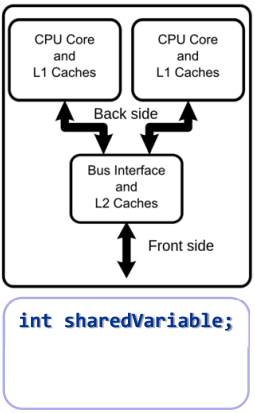
\includegraphics[width=1.5\textwidth]{images/Multicore/Multicore_shared_variable}
\end{minipage}

\paragraph{Kennzeichnung von Variablen mit \lstinline{volatile}}
\begin{itemize}
	\item Alle Variablen, die ausserhalb des Programmkontextes des Prozessors geändert werden können müssen gekennzeichnet werden.
	\item Dies sind:
	\begin{itemize}
		\item Variablen, die speziell bei Embedded Systems ein Hardwareregister darstellen 
		\item Globale Variablen, auf die in mehreren Tasks (concurrency, gleichzeitige Ausführungseinheiten) zugegriffen wird 
		\item Globale Variablen, auf die in Interruptserviceroutinen (ISR) zugegriffen wird
	\end{itemize}
	\item Es muss verhindert werden, das irgendwann mit einer nicht aktuellen Kopie in einem Arbeitsregister gearbeitet wird
\end{itemize}

\subsection{Caches}
\begin{itemize}
	\item Caches sind (für den Prozessor) versteckte schnelle Speicher, die zwischen dem Prozessor und dem Hauptspeicher liegen 
	\item Caches führen eine Kopie von häufig benötigten Hauptspeicherdaten 
	\item Im besten Fall sind die Hauptspeicherdaten, auf welche der Prozessor zugreifen will, bereits im Cache vorhanden.  Dann ist der Speicherzugriff schneller als wenn wirklich auf den Hauptspeicher zugegriffen werden müsste
	\item Bei Multicore Systemen können mehrere Cores je Caches auf dieselben Daten haben, d.h. es kann mehrere Kopien derselben Daten geben 
	\item Cache Coherency: Wie erfährt ein Cache eines Cores, dass ein anderer Core diese Daten geändert hat? \lstinline{volatile} löst das Cache Coherency Problem nicht. Damit wird einzig sichergestellt, dass der Core einen Zugriff Richtung Speicher macht und sich nicht eine Kopie in einem Arbeitsregister hält
\end{itemize}

\subsubsection{Speicherzugriff zur Laufzeit}
\begin{itemize}
	\item \lstinline{volatile} hat Einfluss zur Compile-time und stellt sicher, dass der Compiler keinen Code generiert, bei dem er sich lokale Kopien in einem Register hält. Dank \lstinline{volatile} besteht der Code nun also aus einem expliziten Speicherzugriff  
	\item Dieser Speicherzugriff sollte so schnell wie möglich sein. Hoffnung: die Daten werden in einem möglichst prozessornahen Cache gefunden  
	\item Beim ersten Zugriff auf diese Daten befinden sie sich logischerweise noch nicht im Cache. Ein Geschwindigkeitsgewinn ergibt sich erst ab dem zweiten Zugriff
	\item Triviale Folgerung: Daten, auf die nur einmal zugegriffen werden muss, sollen nicht gecached werden
\end{itemize}

\subsubsection{Lokalität}
\begin{minipage}[t]{6cm}
	\begin{itemize}
		\item Zeitliche Lokalität (Temporal locality) 
		\begin{itemize}
			\item Soeben verwendete Daten oder Instruktionen werden mit hoher Wahrscheinlichkeit bald wieder verwendet 
			\item Caches nutzen die zeitliche Lokalität aus
		\end{itemize}
	\end{itemize}
\end{minipage}
\begin{minipage}[t]{13cm}
	\begin{itemize}
		\item Räumliche Lokalität (Spatial locality) 
		\begin{itemize}
			\item Bei soeben verwendeten Daten oder Instruktionen werden mit hoher Wahrscheinlichkeit auch benachbarte Daten oder Instruktionen bald verwendet 
			\item Die räumliche Lokalität wird in Caches folgendermassen umgesetzt: Wenn auf eine bestimmte Adresse das erste Mal zugegriffen wird, werden nicht nur die Daten von dieser Adresse ins Cache geladen, sondern ein Speicherblock bestimmter Grösse um diese Adresse herum
		\end{itemize}
	\end{itemize}
\end{minipage}

\subsection{Ping Pong Speicher}
Szenario: Ein System empfängt Daten und schriebt diese in einen Buffer. Die Daten werden gefiltert und wieder ausgegeben. Wie kann bei Multicore Systemen verhindert werden, dass der Filterschritt mit inkonsistenten Daten arbeitet? \\
Schlechte Lösung: Buffer wird synchronisiert, oder der Empfangsbuffer wird in einen zweiten Buffer kopiert \\
Gute Lösung: Ping Pong Buffer

\subsubsection{Funktion}
\begin{itemize}
	\item Zwei identische Buffer werden definiert 
	\item Ein Core bestimmt, in welchen Buffer die Daten geschrieben werden 
	\item Nach abgeschlossenem Empfang übergibt der Core dem Filterschritt einen Pointer auf diesen Buffer zur weiteren Bearbeitung 
	\item Dem Empfänger übergibt der Core einen Pointer auf den zweiten Buffer, damit nun in diesen geschrieben wird
	\item Daten werden nicht kopiert, nur Pointer werden von einem Buffer zum anderen hin-und hergewechselt (Ping Pong)
\end{itemize}

